\documentclass[compress]{beamer}
\usepackage{ifthen,verbatim}

\title{Muon-HIP Alignment Workflow}
\author{Jim Pivarski, Alexei Safonov, K\'aroly Banicz$^*$}
\institute{Texas A\&M University, $^*$FermiLab}
\date{ 8 February, 2008}

\newcommand{\isnote}{}
\xdefinecolor{lightyellow}{rgb}{1.,1.,0.25}
\xdefinecolor{lightgrey}{rgb}{0.9,0.9,0.9}
\xdefinecolor{darkblue}{rgb}{0.1,0.1,0.7}

%% Uncomment this to get annotations
%% \def\notes{\addtocounter{page}{-1}
%%            \renewcommand{\isnote}{*}
%% 	   \beamertemplateshadingbackground{lightyellow}{white}
%%            \begin{frame}
%%            \frametitle{Notes for the previous page (page \insertpagenumber)}
%%            \itemize}
%% \def\endnotes{\enditemize
%% 	      \end{frame}
%%               \beamertemplateshadingbackground{white}{white}
%%               \renewcommand{\isnote}{}}

%% Uncomment this to not get annotations
\def\notes{\comment}
\def\endnotes{\endcomment}

\setbeamertemplate{navigation symbols}{}
\setbeamertemplate{headline}{\mbox{ } \hfill
\begin{minipage}{5.5 cm}
\vspace{-0.75 cm} \small
\end{minipage} \hfill
\begin{minipage}{4.5 cm}
\vspace{-0.75 cm} \small
\begin{flushright}
\ifthenelse{\equal{\insertpagenumber}{1}}{}{Jim Pivarski \hspace{0.2 cm} \insertpagenumber\isnote/\pageref{numpages}}
\end{flushright}
\end{minipage}\mbox{\hspace{0.2 cm}}\includegraphics[height=1 cm]{../cmslogo} \hspace{0.1 cm} \includegraphics[height=1 cm]{../tamulogo} \hspace{0.01 cm} \vspace{-1.05 cm}}

\begin{document}
\frame{\titlepage}

%% \begin{notes}
%% \item This is the annotated version of my talk.
%% \item If you want the version that I am presenting, download the one
%% labeled ``slides'' on Indico (or just ignore these yellow pages).
%% \item The annotated version is provided for extra detail and a written
%% record of comments that I intend to make orally.
%% \item Yellow notes refer to the content on the {\it previous} page.
%% \item All other slides are identical for the two versions.
%% \end{notes}

\begin{frame}
\frametitle{Two projects}
\hspace{-0.83 cm} \textcolor{darkblue}{Very early alignment of muon endcaps}

\vspace{-0.25 cm}
\begin{columns}
\column{0.8\linewidth}
\begin{itemize}\setlength{\itemsep}{0.25 cm}
\item Align chambers and layers relative to each other with beam-halo (before
first collisions) through CSC overlap hits
\item Align whole rings relative to the tracker with several hundred I.P.\ muons
\item Two opportunities to compare~with~hardware~alignment~\mbox{\hspace{-10 cm}}
\item Manually configured and operated by~K\'aroly~Banicz~and~me~\mbox{\hspace{-10 cm}}
\end{itemize}
\column{0.2\linewidth}
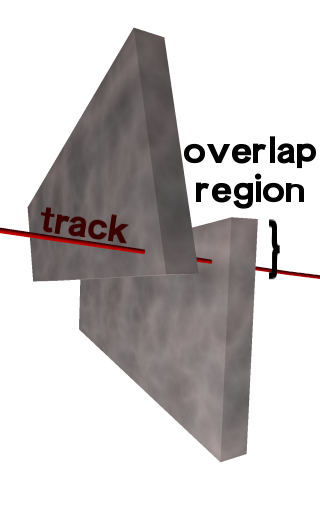
\includegraphics[width=\linewidth]{overlap.png}

\vspace{1 cm}
\mbox{ }
\end{columns}

\vfill
\hspace{-0.83 cm} \textcolor{darkblue}{10 to 100~pb$^{-1}$ alignment of the whole muon system}

\begin{columns}
\column{\linewidth}
\begin{itemize}\setlength{\itemsep}{0.25 cm}
\item Align chambers relative to the tracker with tens of thousands
through millions of I.P.\ muons
\item Automated and parallelized, run on the CAF
\end{itemize}
\column{0 cm}
\end{columns}

%% \hspace{-0.83 cm} \textcolor{darkblue}{\Large Outline2}
\end{frame}

\begin{frame}
\frametitle{Very early alignment of endcaps}
\begin{itemize}
\item See K\'aroly's talk at yestday's CSC DPG
\item Alternate between track-fitting even-numbered chambers, aligning odd, and fitting odd, aligning even
\begin{center}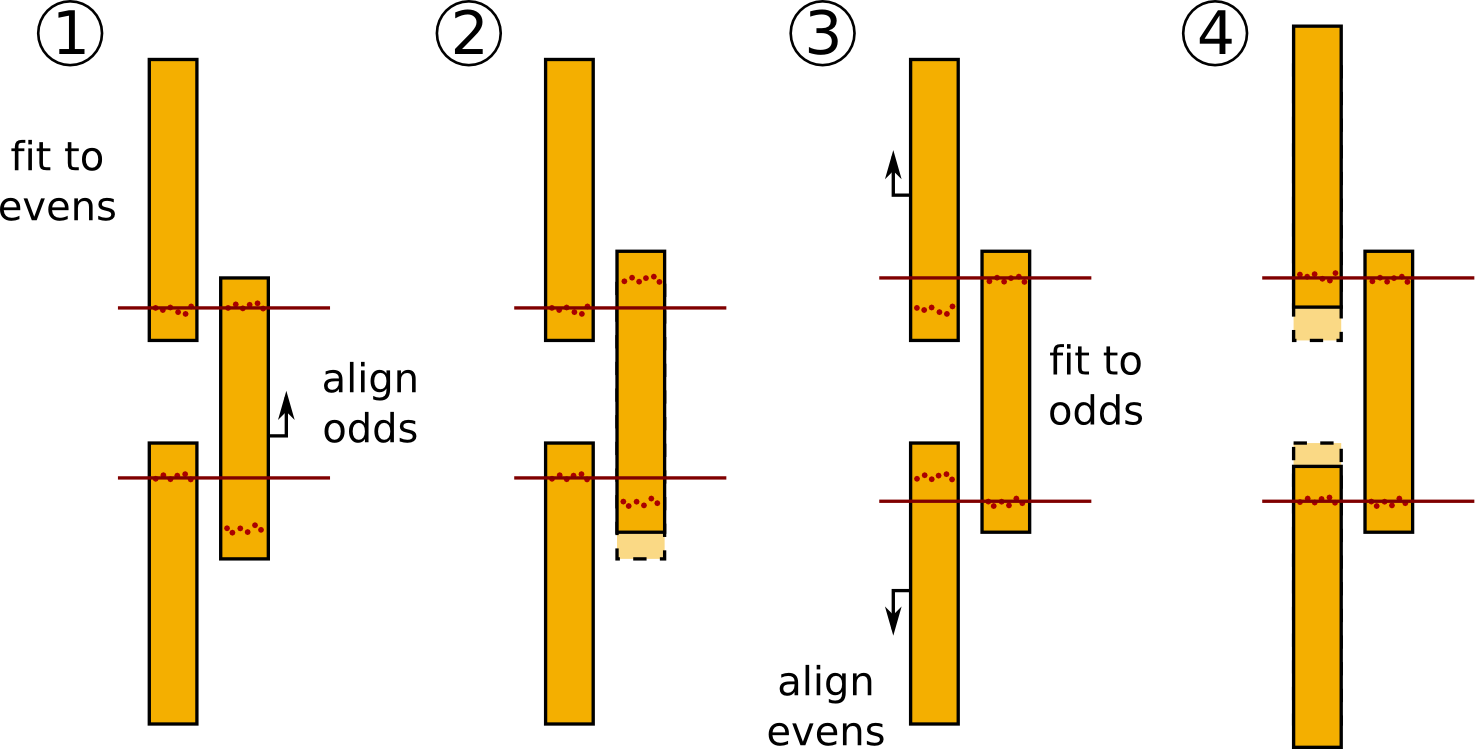
\includegraphics[width=0.65\linewidth]{beamhalo.png}\end{center}

\vfill
\item Ring alignment step requires a new level in muon hierarchy
\begin{center}\ldots $\to$ CSCStations $\to$ \textcolor{blue}{CSCRing} $\to$ CSCChamber $\to$ \ldots\end{center}

\item New item since last meeting
\begin{itemize}
\item Hard to implement a structural change like this for 2\_0\_0?
\item I'd like to have that discussion offline
\end{itemize}
\end{itemize}
\end{frame}

\begin{frame}
\frametitle{Workflow for 10 and 100~pb$^{-1}$}
\begin{itemize}
\item 9 passes, the first having 15 iterations, the rest 5 (total of 55)
\begin{itemize}
\item First align wheels and disks, slow convergence
\item Next align innermost muon stations
\item Then fix innermost and align next, etc.
\item Then allow everything to float when close to optimum
\end{itemize}
\item Data selected by a $p_T$ cut and a new track cut that rejects highly-scattering tracks
\end{itemize}

\vfill
\hspace{-0.83 cm} \textcolor{darkblue}{\Large Resources for 100~pb$^{-1}$}
\begin{itemize}
\item Assuming all $W+Z$ and no QCD: 714,000 events
\item 54 CPUs + 1 control job
\item 11 min/iter $\to$ 10 hours wall time \textcolor{blue}{(ideally)}
\item 12 MB/iter output on {\it local} disk $\to$ 660 MB
\item Typical max memory: 300 MB, max swap: 700 MB
\item \textcolor{blue}{CASTOR failed on 13 jobs (0.6\%), each of which pauses the entire process--- must be restarted by hand}
\end{itemize}
\end{frame}

\beamertemplateshadingbackground{lightgrey}{white}
\begin{frame}
\frametitle{Implementation details (skip?)}
\begin{itemize}\setlength{\itemsep}{0.3 cm}
\item Single perl script creates all necessary directories and
configuration files; easy to stop and restart a half-finished job
\item One control job submits parallel sub-processes, waits for them to finish
\begin{itemize}
\item This CPU spends most of its time sleeping
\item Waits forever if sub-job fails
\end{itemize}

\item Muon geometry is passed from one iteration to the next via
SQLite files: last one copied into database by hand

\item Residuals monitoring through CommonAlignmentMonitor

\item Alignment monitoring through MuonGeometryIntoNtuples

\item For MC, combine datasets at the level of parameter matrices
(individual subjobs run on pure samples)
\end{itemize}
\end{frame}
\beamertemplateshadingbackground{white}{white}

\begin{frame}
\frametitle{Work to be done}
\textcolor{darkblue}{Relative chamber alignment with beam-halo:}
\begin{itemize}\setlength{\itemsep}{0.2 cm}
\item Need HLT paths for beam-halo technical trigger
\item CSC overlap hits need to be put on CosmicMuon tracks
\item Need to submit code for setting APEs (through CommonAlignmentMonitor)
\item Need to write and submit geometry-monitoring scripts
\item Need to test survey constraints for muon system
\item Develop procedure on MC (beam-halo rate is ``factor-of-100''
uncertain: level of feasibility will not be fully known)
\end{itemize}

\vfill
\textcolor{darkblue}{Ring alignment with globalMuon tracks:}
\begin{itemize}\setlength{\itemsep}{0.2 cm}
\item Need to add CSCRing level of hierarchy
\item Need to submit track-scattering cut
\end{itemize}
\end{frame}

\begin{frame}
\frametitle{Work to be done}
\textcolor{darkblue}{10 and 100~pb$^{-1}$ full alignments:}
\begin{itemize}\setlength{\itemsep}{0.25 cm}
\item Procedure runs, but with CASTOR problems (now rare, but still a problem)
\item Same new code requirements
\item Determine optimal cut and preferred parameters for AlCaReco

(to be coordinated with MillePede muon alignment group)
\item Systematics studies (in 1\_6\_7 with large data samples)
\begin{itemize}
\item Still need to try several configurations (optimize new track cut)
\item Miscalibrations, misaligned tracker, wrong $\rho(\vec{x})$, $\vec{B}(\vec{x})$\ldots
\item Generic event selection with $p_T$ cut, rather than $W$, $Z$
\item Layer alignment feasibility study
\end{itemize}
\item CSA08: make sure the baseline procedure works and gives the same results in CMSSW\_2\_0\_0
\begin{itemize}
\item Need small 2\_0\_0 $Z\to\mu\mu$ sample: 54,000 events after AlCaRecoMu cuts
\end{itemize}
\end{itemize}
\end{frame}

\begin{frame}
\frametitle{Conclusions}
\textcolor{darkblue}{Requests:}
\begin{itemize}
\item More reliable CASTOR access
\item Occasional overnight use of 50 CPUs
\item Larger non-CASTOR space?  (several GB)
\end{itemize}

\vfill
\textcolor{darkblue}{Status:}
\begin{itemize}
\item Baseline 100~pb$^{-1}$ procedure is almost in good shape: \\ early
tests show 300--800~$\mu$m, depending on station
\item Finished 85\% of a full walkthrough, with manual intervention
\item A lot of new code to submit; most of it is written
\begin{itemize}
\item We need to talk about new item: CSCRing
\end{itemize}
\end{itemize}

\vfill
\textcolor{darkblue}{CSA08:}
\begin{itemize}
\item Extensive physics-tests of the procedure using 1\_6\_7 and existing CSA07 samples
\item Check that software still works in 2\_0\_0 and beyond
\end{itemize}

\label{numpages}
\end{frame}

\end{document}
